\clearpage
\section{The Tangent Function}
The tangent is a bit different than the sine and cosine. It \textit{is} a basic trigonometric function, and \textit{is} defined by sides of a right triangle, it does not follow the same up and down wave pattern.

The tangent of an angle is defined as the ratio of the opposite and adjacent sides of a right triangle. It is also expressed as the sine function divided by the cosine function.
\begin{center}
    \begin{minipage}[c]{0.4\linewidth}
        \centering
        \begin{tikzpicture}
            \begin{axis}[%
                xmin = -0.3, xmax = 1.1,
                ymin = -0.3, ymax = 1.1,
                axis lines = none,
                width = \linewidth, height = \linewidth
            ]
            
            \draw[red, thick] (0,0) -- (1,0) node[midway, below, black] {adj};
            \draw[blue, thick] (1,0) -- (0,1) node[midway, above right, black] {hyp};
            \draw[red, thick] (0,0) -- (0,1) node[midway, left, black] {opp};
            
            \node[right] at (0.65, 0.1) {$\theta$};
            \draw[color = black, thick] (0.8,0) arc (180:135:0.2);
            
            \draw[thick, color = black] (0,0.1) -- (0.1,0.1) -- (0.1,0);
            \end{axis}
        \end{tikzpicture}
    \end{minipage}%
    \begin{minipage}[c]{0.3\linewidth}
        \begin{align*}
            \tan(\theta) &= \frac{opposite}{adjacent} \\
            \tan(\theta) &= \frac{\sin(\theta)}{\cos(\theta)}
        \end{align*}
    \end{minipage}
\end{center}
Let's look at the graph of the tangent function, but it's quite different from the sine and cosine.
\begin{center}
    \begin{minipage}[c]{0.33\linewidth}
        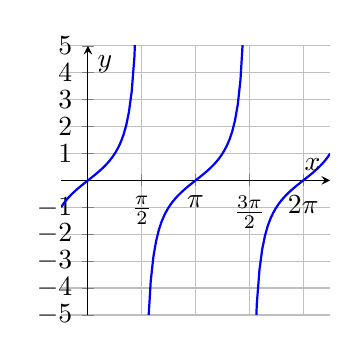
\begin{tikzpicture}
            \begin{axis}[%
                xlabel = {$x$}, ylabel = {$y$},
                xmin = -1 * 0.25 * pi,, xmax = (9 * pi) / 4,
                ymin = -5, ymax = 5,
                restrict y to domain=-10:10,
                xtick = {
                    0, 
                    pi / 2, 
                    pi, 
                    (3 * pi) / 2,
                    2 * pi%
                    },
                xticklabels = {
                    $0$,
                    $\frac{\pi}{2}$,
                    $\pi$,
                    $\frac{3\pi}{2}$,
                    $2\pi$%
                },
                ytick = {
                    -5,
                    -4,
                    -3,
                    -2,
                    -1,
                    1,
                    2,
                    3,
                    4,
                    5%
                },
                axis lines = center, grid = both,
                width = 5cm, height = 5cm,
                trig format plots=rad
            ]
            \addplot[color = blue, thick, domain = -1 * 0.25 * pi:9/4*pi, samples = 100]{tan(x)};
            \end{axis}
        \end{tikzpicture}
    \end{minipage}
    \begin{minipage}[c]{0.66\textwidth}
        At left is $f(x) = \tan(x)$ graphed on the $xy$-plane, where $x$ is an angle in radians. There are some things to note about this function.
        \begin{itemize}
            \item Unlike the sine and cosine functions, there are asymptotes in this function. They appear when $x = \frac{\pi(2n + 1)}{2}$, where $n$ is an integer (i.e. $1,2,3,4,\text{etc.}$)
        \end{itemize}
    \end{minipage}
\end{center}
The notation $\frac{\pi(2n + 1)}{2}$ indicates that the numerator is always $\pi$ multiplied by an odd number. These values include:
\begin{align*}
    n = 1&: \frac{\pi}{2} \\
    n = 2&: \frac{3\pi}{2} \\
    n = 3&: \frac{5\pi}{2} \\
    n = a&: \frac{\pi(2a + 1)}{2} && \text{$a$ is an arbitrarily large integer}
\end{align*}
We could also say that $n$ is an odd integer (i.e. $1,3,5,7,\text{etc.}$) like we did in the cosine section.

To understand why, remember that the tangent function is defined as the sine function divided by the cosine function. That means $\cos(x)$ is in the denominator.

From the section on the cosine function, we know that $\cos(x)$ has zeroes when $x = \frac{\pi(2n + 1)}{2}$. As a result, tangent is not continuous/undefined at those values of $x$.

As for why the function shoots up to infinity when it gets close to those $x$ values, recall what happened when we plugged smaller and smaller values into the function $g(x) = \frac{1}{x}$ back when we first covered asymptotes. The smaller the denominator got, the large the output got. For example:
\begin{align*}
    g(0.000000001) &= \frac{1}{0.000000001} = 1000000000 \\
    g(-0.000000001) &= -\frac{1}{0.000000001} = -1000000000
\end{align*}
The same is happeneing in this function. As the angle (in radians) gets closer to, say, $\frac{\pi}{2}$, $\sin(x)$ gets closer and closer to $1$ and $\cos(x)$ gets closer and closer to $0$. When this happens, what we get is something like this:
\begin{align*}
    \tan\left(\frac{\pi}{2} - 0.0001 \right) &= \frac{\sin\left(\frac{\pi}{2} - 0.0001 \right)}{\cos\left(\frac{\pi}{2} - 0.0001 \right)}
    \approx \frac{0.9999999999}{0.00001} \approx 99999.999\dots \\
    \tan\left(\frac{\pi}{2} + 0.0001 \right) &= \frac{\sin\left(\frac{\pi}{2} + 0.0001 \right)}{\cos\left(\frac{\pi}{2} + 0.0001 \right)}
    \approx \frac{0.9999999999}{-0.00001} \approx -99999.999\dots
\end{align*}
\begin{itemize}
    \item Tangent has zeroes at $x = n\pi$, where $n$ is an integer (i.e. $1,2,3,4,\text{etc.}$)
\end{itemize}
This is true for the same reason as the previous. In the definition of the tangent function, $\sin(x)$ is in the numerator. From the sine section, we learned that $\sin(x) = 0$ when $x = n\pi$, so $\frac{0}{anything} = 0$.
\clearpage
With everything we have, we can say the following about the domain and range:
\begin{align*}
    x \neq \frac{\pi(2n + 1)}{2} \\
    y \in (-\infty, \infty)
\end{align*}
Or, if we wanna get fancy, we can use:
\[
    \text{Domain}: \left\{ x \mid x \neq \frac{\pi(2n + 1)}{2}, n \in \mathbb{Z} \right\} \\
\]
This is called \textbf{set-builder} notation. It just means that $x$ cannot equal $\frac{\pi(2n + 1)}{2}$ where $n$ is an integer. $\mathbb{Z}$ is the set of all integers. So if $n$ is in the set of all integers, then it's also an integer. 

But don't worry about that notation. I never saw set-builder notation in Calculus II and, while I \textit{have} seen it in Calculus III, I've never had to write one myself. Your teacher/professor will not expect you to know this, and you probably won't touch it for a \textit{while}. It's pretty cool to know, though.
\clearpage